%===============================================================================
% Brno University of Technology
% Faculty of Information Technology
% Academic year: 2018/2019
% Bachelor thesis: Monitoring Pedestrian by Drone
% Author: Vladimir Dusek
%===============================================================================

\chapter{Přehled dronů a jejich srovnání}
\label{chap_3}

Dron, nebo také bezpilotní letadlo (UAV~--~\textit{unmanned aerial vehicle}), je létající objekt, který nemá posádku. Může být ovládaný na dálku, mít předprogramovanou trasu letu nebo využívat složitější dynamické autonomní systémy. Nejčastější jsou dálkové modely letadel, vrtulníků a multikoptér. Naváděné střely, ačkoliv jsou bezpilotní a v~některých případech řízeny vzdáleně, nejsou klasifikovány jako UAV, protože tyto zbraně jsou pouze na jedno použití~\cite{wikiDrone}.

Pokud člověk létá s~jakýmkoliv dronem, stává se účastníkem leteckého provozu a musí dodržovat jistá pravidla. Létání je třeba provozovat v~bezpečné vzdálenosti od lidí. Srážky jistých modelů s~člověkem mohou mít závažné zdravotní následky. Také je nutné vyhnout se leteckému provozu~--~je zakázáno létat v~blízkosti letišť a celkově létat výše než 300 metrů nad zemí. Nelze také létat v~zakázaném leteckém prostoru (bezletové zóně)~\cite{wikiDrone}.

Počátky bezpilotních letounů sahají k~počátkům 20. století. Už ve 20. letech se stroje začínaly podobat dnešním dronům, ačkoliv disponovaly podstatně většími rozměry. Původně měly sloužit hlavně pro přepravu lidské posádky, to ale nezaznamenalo výraznější úspěch. Postupem času se jejich oblast využítí změnila. Dnes obvykle nesou kamery, termokamery či jiná monitorovací zařízení, kterými poskytují při leteckém snímkování důležitá data pro nejrůznější účely~\cite{wikiDrone}.

%===============================================================================

\section{Využití dronů}
\label{sec_drones_usage}

Dnes se nejčastěji setkáváme s~malými drony, které jsou dálkově ovládané a oblast jejich využití je velmi široká~\cite{articleDroneUsage}. Stavební firmy je používají pro monitorování důležitých infrastruktur, ropovodů nebo dálnic. V~energetice se pomocí dronů a speciálních kamer měří elektrické vedení. Ve filmové či hudební produkci se pomocí dronů natáčejí záběry ze vzduchu. Drony také zvládají 3D mapování povrchu, díky čemuž se vytváří geografické modely a mapy. Využívat se dají i v~zemědělství, například při sledování kvality hnojení nebo osevu. Bezpilotní letadla se používají v~armádě k~průzkumným i útočným letům.

Drony jsou také skvělou pomůckou v~oblasti bezpečnosti. Záchranáři je mohou využívat pro rychlé vyhledání nehody, policie pro sledování a průzkum terénu, hasiči pro zachycení velikosti požáru, či dokonce k~jeho hašení. V~oblasti zabezpečení areálů se drony používají k~monitorování oblastí. Mohou také posloužit pro kontrolování a focení těžko dostupných míst, například větrných elektráren, určitých typů střech apod. Nahraná dokumentace z~dronu může posloužit jako důkazní materiál.

%===============================================================================

\section{Dostupné drony na trhu}

To, jak dron vypadá, kolik stojí a jaké má rozměry, samozřejmě záleží od účelu využití, ke kterému byl konstruován. Největší a nejdražší jsou armádní bojové drony~--~bezpilotní letouny. Ty disponují rozpětím křídel až desítkami metrů a stojí v~přepočtu stovky miliónů korun. Mají velkou dráhu doletu a vysokou vzletovou výšku. Může jít o~ozbrojené drony, s~nimiž armáda likviduje cíle, aniž by byly ohroženy životy pilotů, nebo mohou sloužit k~rozsáhlým špionážním akcím~\cite{articleDroneUsage}.

Filmařské drony jsou samozřejmě vybaveny kvalitní nahrávací technikou. Disponují obvykle několika vrtulemi pro zajištění větší stability. Příchod dronů změnil styl novodobého natáčení leteckých scén. Pronájem, potažmo koupě reálného vrtulníku, je samozřejmě vysoce nákladná záležitost, letecké záběry se tak staly mnohonásobně dostupnější. Cena špičkových filmařských dronů se pohybuje v~řádech sta tisíců korun~\cite{articleDroneUsage}.

Donáškové drony jsou zatím spíše futuristická záležitost. Zahraniční technologické firmy, jako Amazon nebo Google, již testují své služby~\cite{droneDelivery}. Zboží o~váze několik kilogramů chtějí rozvážet menšími vrtulovými drony. Problém ani tak není technologický vývoj, ale zákony. V~současnosti ve většině světa není takovýto způsob dopravy zboží legislativně nijak ošetřen. Jde však pravděpodobně o~otázku času, než se začnou donáškové drony využívat.

Komerční drony stojí řádově desítky tisíc korun a jsou tak cenově nejdostupnější. Lze s~nimi snadno manévrovat a dokáží pořizovat dostatečně kvalitní záběry pro běžnou spotřebu. Oblíbené tak jsou u~cestovatelů, kteří dokáží ocenit především panoramatické záběry, na které by jinak neměli nárok, tak u~leteckých nadšenců a amatérských pilotů. Několik konkrétních modelů je popsáno ve zbytku této kapitoly~\cite{articleDji}.

\begin{figure}[H]
    \centering
    \begin{tabular}{cc}
        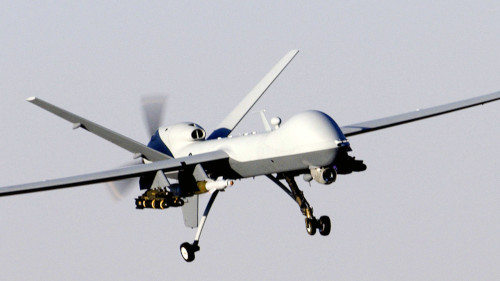
\includegraphics[width=.375\textwidth]{drone-military.jpg} &
        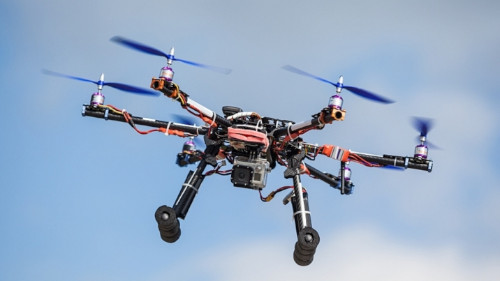
\includegraphics[width=.375\textwidth]{drone-film.jpg} \\
        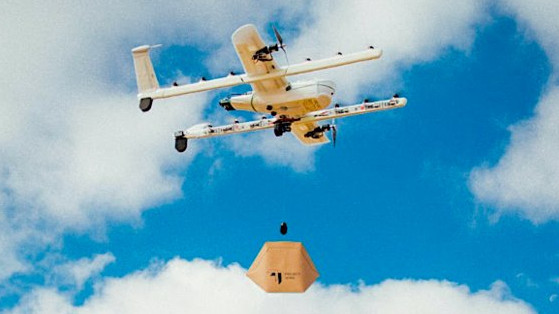
\includegraphics[width=.375\textwidth]{drone-delivery.jpg} &
        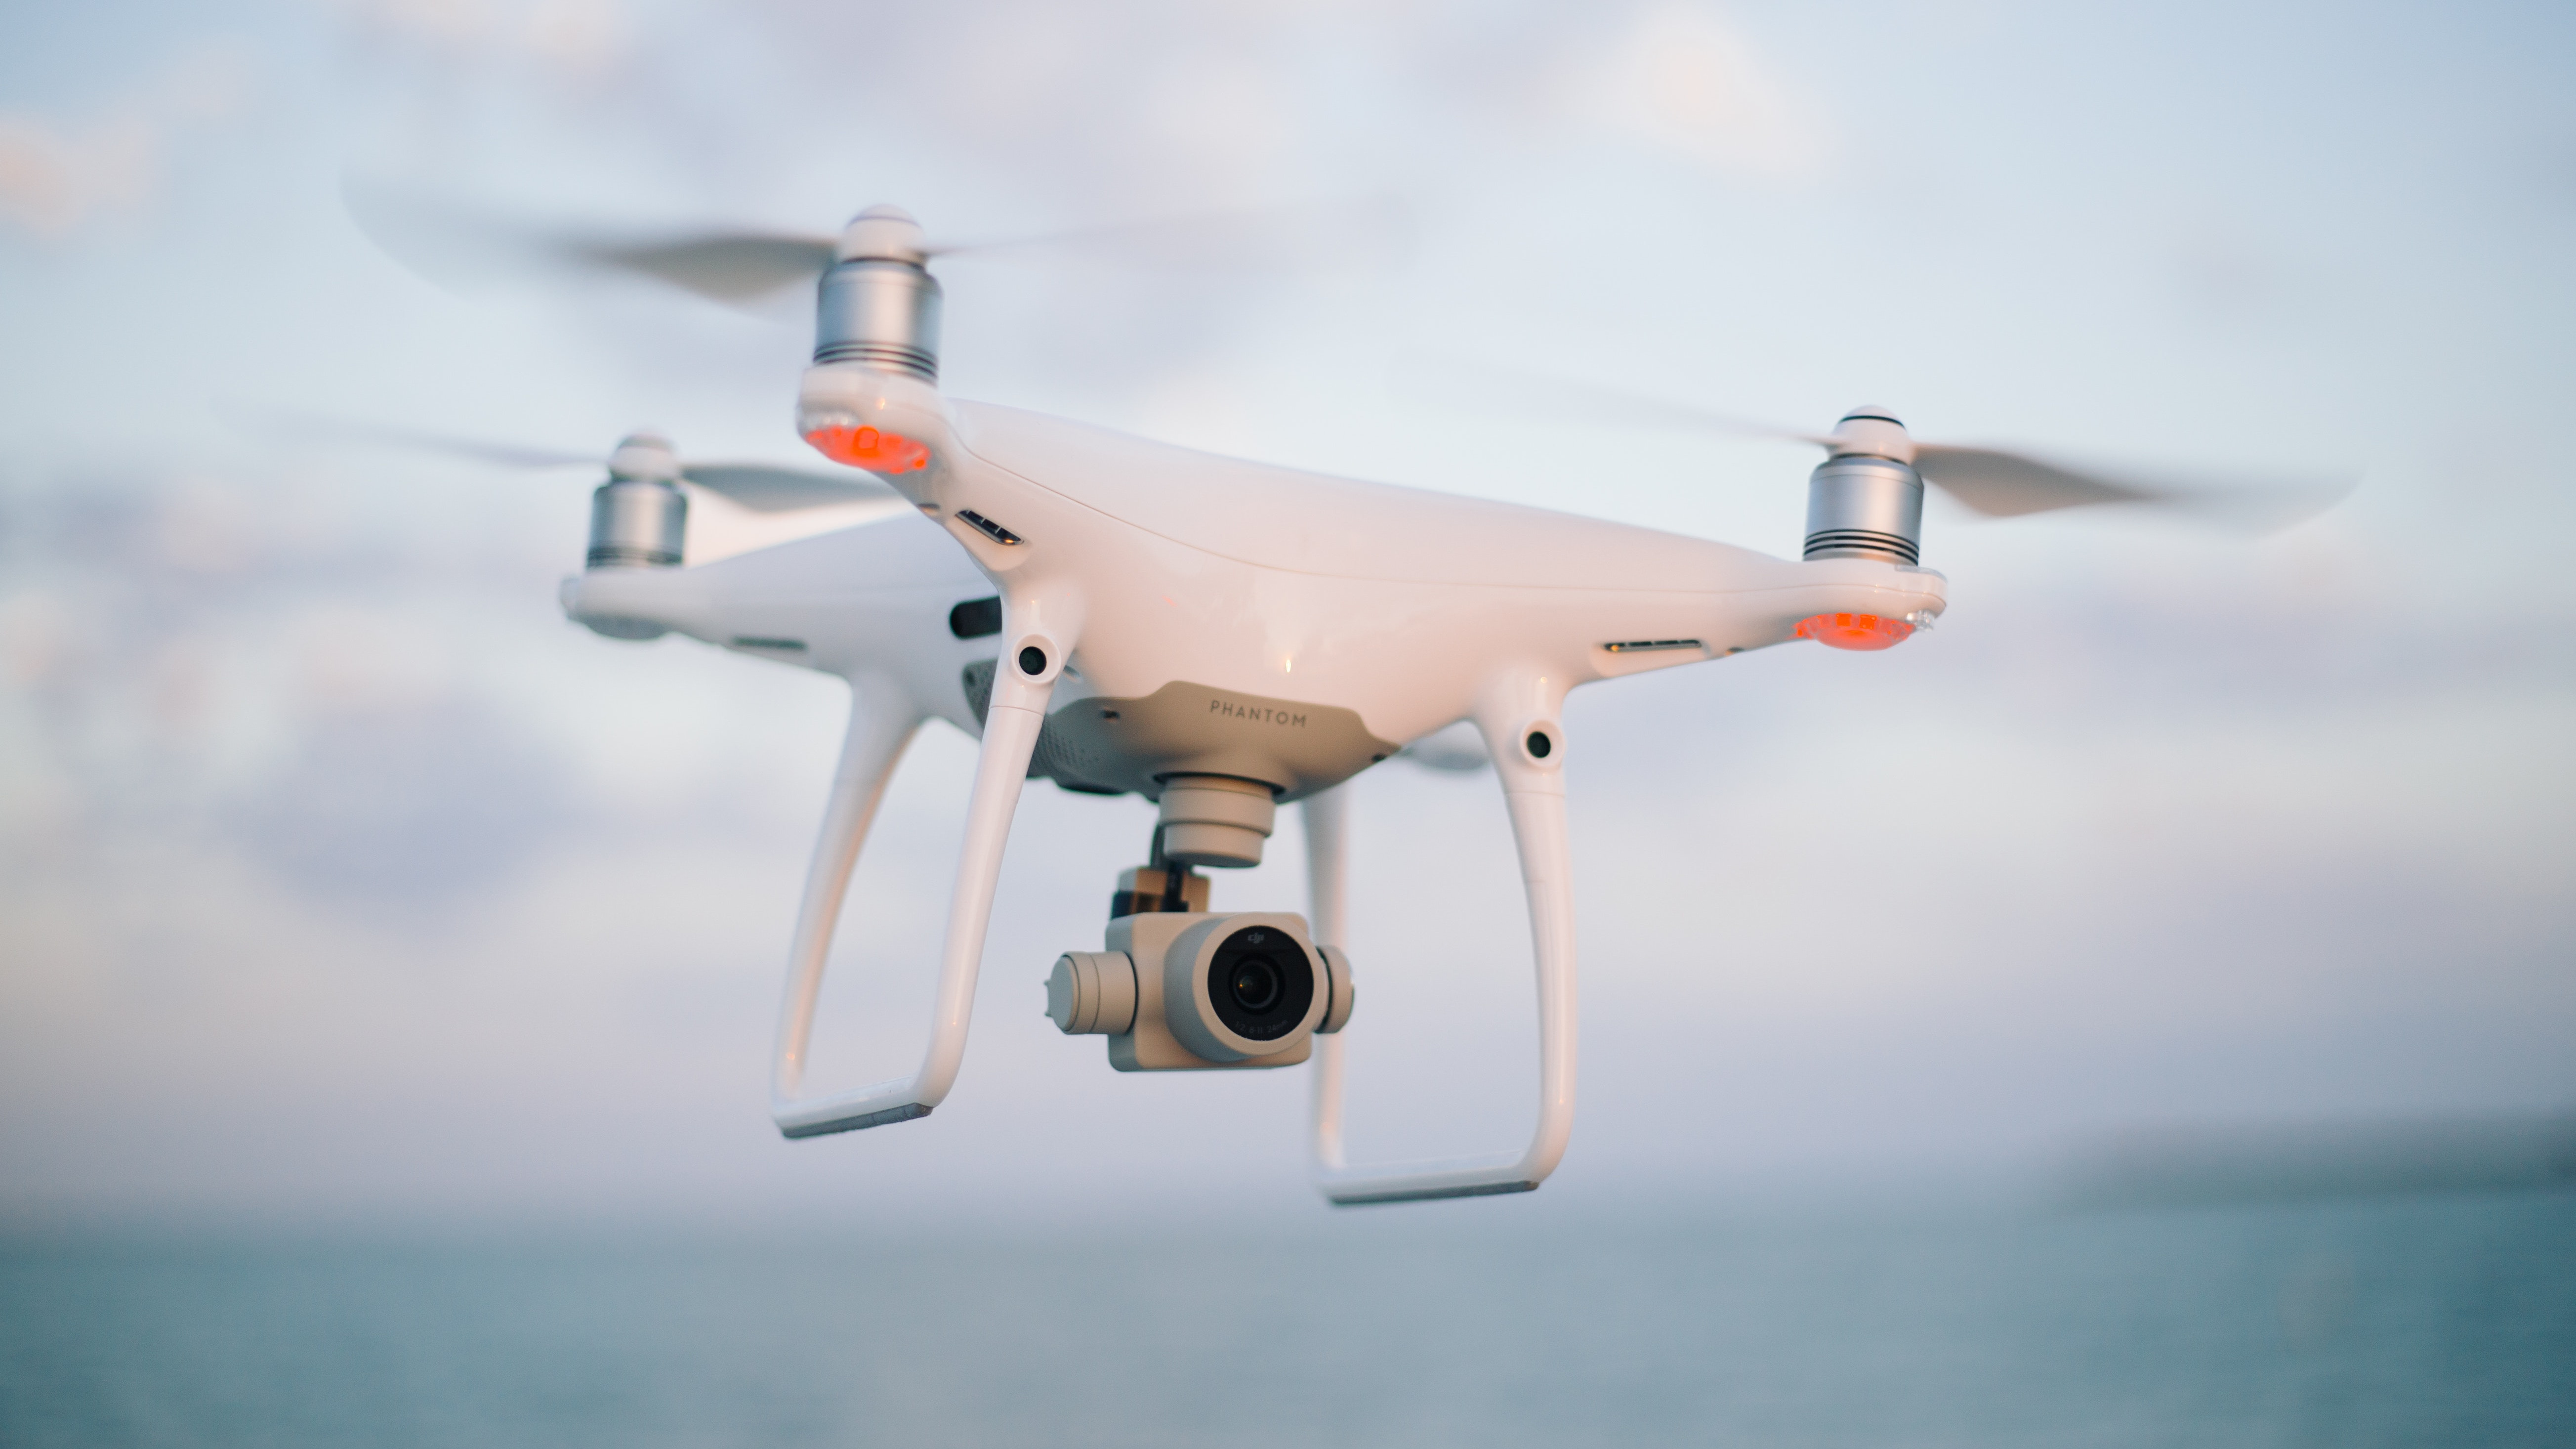
\includegraphics[width=.375\textwidth]{drone-commercial.jpg} \\
    \end{tabular}
    \caption[Ukázky dronů podle typu použití]{Ukázky dronů podle typu použití. Armádní, filmařský, doručovací a komerční dron. Obrázky jsou převzaté~\cite{wikiDrone, droneDelivery}.}
    \label{fig_drones}
\end{figure}

%-------------------------------------------------------------------------------

\pagebreak

\subsection*{DJI Mavic~2~Pro}

Čínská firma DJI je v~současnosti nejzvučnější jméno v~oblasti civilních dronů. Produkují několik odlišných řad, pro různé cílové skupiny. Inovují, udávají trendy a v~současnosti pokrývají asi 70\% trhu~\cite{articleDji}.

Mavic~2~Pro je nástupce velmi úspěšného dronu Mavic~Pro. Váží 907\,g, dokáže létat rychlostí až 72\,km\,/\,h a ve vzduchu vydrží až 31~minut. Dá se ovládat až do vzdálenosti 18\,km. Má špičkovou kameru s~rozlišením 20\,MP, která dokáže natáčet video až ve 4\,K rozlišení a v~60 snímcích za vteřinu. Nabízí spoustu módů pro natáčení a focení, například \textit{hyperlapse} pro stabilizované časosběrné záznamy. Dron se dá složit do kompaktních rozměrů~--~$214 \times 91 \times 84$\,mm). Mezi komerčními drony se jedná o~drona z~vyšší cenové kategorie, pořizovací cena je 1\,500\,\$. Technické parametry jsou převzaté z~oficiálních stránek výrobce~\cite{specsMavic2}.

\begin{figure}[H]
    \centering
    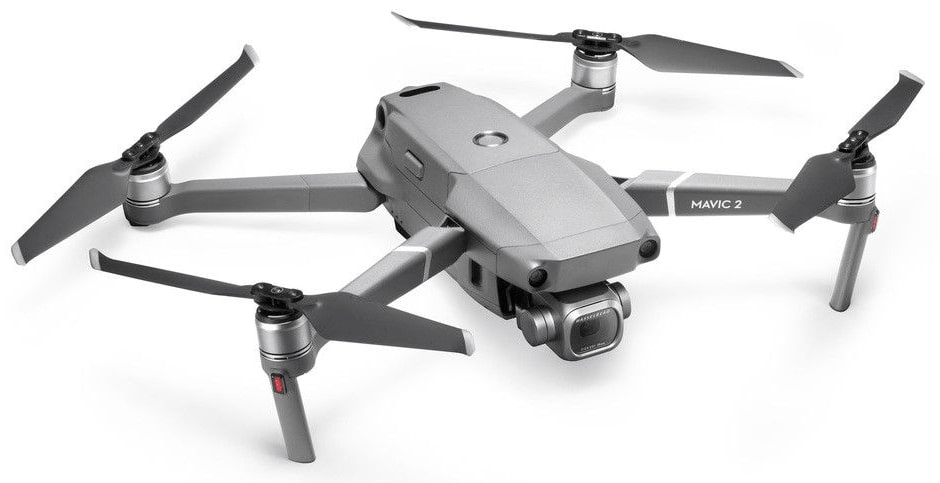
\includegraphics[width=0.8\linewidth]{dji-mavic-pro.jpg}
    \caption[DJI Mavic 2 Pro]{DJI Mavic 2 Pro. Obrázek je převzatý~\cite{specsMavic2}.}
    \label{fig_dji-mavic-pro}
\end{figure}

S~ohledem na monitorování chodců se jedná o~ideálního drona. Důležité jsou zejména kvalitní snímky ve vysokém rozlišení, které umožní lidi ve videu lépe identifikovat. Čím vyšší rozlišení, tím z~větší výšky je možné chodce spolehlivě detekovat. Výdrž baterie se dá považovat za limitující, bohužel v~současné době je toto technologické maximum. Žádná konkurence nenabízí výrazně delší výdrž. Dosah letu až 18\,km je naprosto dostačující, i s~ohledem na maximální dobu letu.

%-------------------------------------------------------------------------------

\pagebreak

\subsection*{DJI Spark}

Spark je malý, lehký, kompaktní dron, kterého není problém strčit do batohu či dokonce kapsy od bundy. Váží pouhých 300\,g, je schopen nabrat rychlost až 50\,km\,/\,h a létat vydrží 16~minut. Dosah doletu je 2\,km v~ideálních podmínkách. Kamera má rozlišení 12\,MP a je schopna natáčet video v~rozlišení Full~HD ve~30 snímcích za~vteřinu. Spark se pohybuje v~jiné cenové kategorii než Mavic~2~Pro a stojí 500\,\$. Technické parametry jsou převzaté z~oficiálních stránek výrobce~\cite{specsSpark}.

\begin{figure}[H]
    \centering
    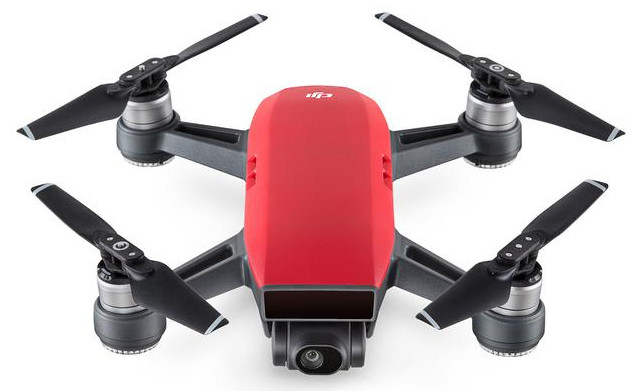
\includegraphics[width=0.75\linewidth]{dji-spark.jpg}
    \caption[DJI Spark]{DJI Spark. Obrázek je převzatý~\cite{specsSpark}.}
    \label{fig_dji-spark}
\end{figure}

Spark není dron pro náročné piloty. Jedná se spíše o~rodinného drona, který je snadný na ovládání a může dobře posloužit například pro focení na dovolené. Spark je $3 \times$ levnější než Mavic Pro, daň za to je nižší výdrž baterie a horší kvalita videa. Je to pochopitelné, cílová skupina obou dronů je rozdílná. Pro monitorování chodců se samozřejmě dá použít, ale všechny jeho kompromisy jsou v~tomto ohledu na škodu. Rozlišení omezí výšku, ze které by bylo možné osoby detekovat. Kapacita baterie zase dobu, po kterou je možné monitorování realizovat. Spark má také výrazně kratší doletovou vzdálenost.

%-------------------------------------------------------------------------------

\pagebreak

\subsection*{Parrot Bebop 2}

Dron od francouzské společnosti Parrot~SA. Narozdíl od předchozích dronů od společnosti DJI, se Bebop~2 ovládá pomocí aplikace v~chytrém telefonu nebo tabletu. Váží 500\,g, dokáže létat rychlostí až 60\,km\,/\,h a ve vzduchu vydrží až 25 minut. Maximální dosah letu je pouhých 300\,m. Má 14\,MP čočku kamery a zvládne pořizovat videozáznam v~rozlišení Full~HD při 30~snímcích za sekundu. Jedná se o~drona ze stejné cenové kategorie jako DJI Spark a pořizovací cena se pohybuje kolem 500\,\$. Technické parametry jsou převzaté z~oficiálních stránek výrobce~\cite{specsParrot}.

\begin{figure}[H]
    \centering
    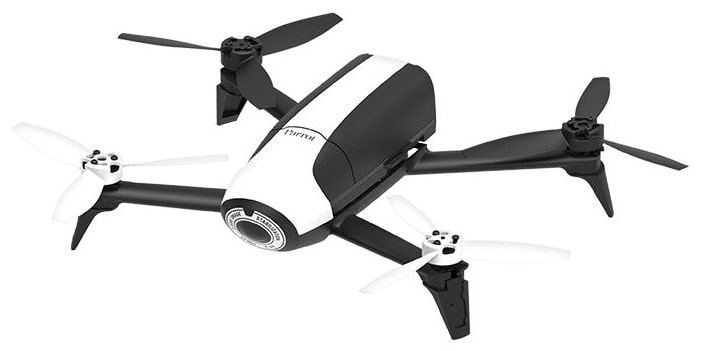
\includegraphics[width=0.85\linewidth]{bebop-2.jpg}
    \caption[Parrot Bebop 2]{Parrot Bebop 2. Obrázek je převzatý~\cite{specsParrot}.}
    \label{fig_bebop-2}
\end{figure}

Bebop~2 se dá považovat za konkurenta Sparka. Je těžší a větší, díky tomu má větší kapacitu baterie a vydrží létat delší dobu. V~letové rychlosti a ceně jsou na tom se Sparkem velmi podobně. Bebop~2 má ale nízký maximální dolet. To by při monitorování mohlo být limitující, pilot by se musel nacházet velmi blízko u~monitorované oblasti. Rozlišení pořízovaného záznamu je shodné, takže platí to co u~Sparka.

%===============================================================================
